\documentclass{article}
\usepackage[T1]{fontenc}
\usepackage{helvet}
\renewcommand{\familydefault}{\sfdefault}
\usepackage{amsmath,amssymb}
\usepackage{sansmath}
\usepackage{tikz}
\usetikzlibrary{arrows.meta,fit,calc,positioning}
\pagestyle{empty}
\definecolor{acc}{HTML}{1F4E79}
\newsavebox{\figbox}
\begin{document}
\sansmath\fontsize{7}{8.4}\selectfont
\sbox{\figbox}{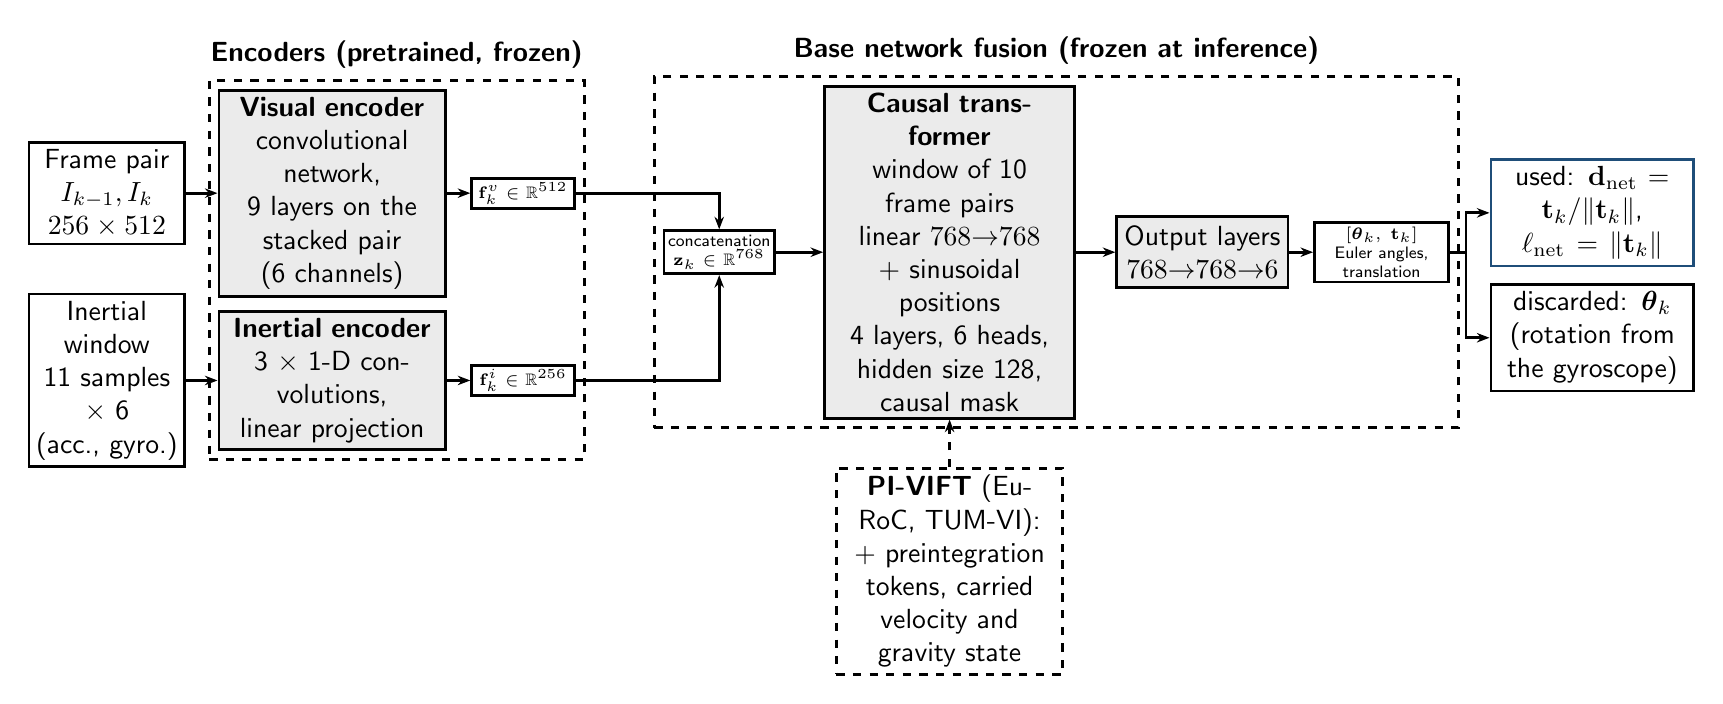
\begin{tikzpicture}[>={Stealth[length=1.6mm]}, every path/.style={line width=1pt}, node distance=4mm,
  blk/.style={draw, align=center, inner sep=2.5pt, minimum height=9mm, text width=#1},
  blk/.default=22mm,
  inp/.style={blk=18mm},
  enc/.style={blk=27mm, fill=black!8},
  tf/.style={blk=30mm, fill=black!8, minimum height=22mm},
  ten/.style={draw, align=center, inner sep=1.5pt, font=\fontsize{6}{7}\selectfont, text width=#1},
  ten/.default=12mm,
  use/.style={blk=24mm, draw=acc},
  var/.style={blk=27mm, dashed},
  lab/.style={font=\bfseries}]
\node[inp] (imgs) {Frame pair\\$I_{k-1}, I_k$\\$256\times512$};
\node[inp, below=6mm of imgs] (imus) {Inertial window\\11 samples $\times$ 6\\(acc., gyro.)};
\node[enc, right=of imgs] (venc) {\textbf{Visual encoder}\\convolutional network,\\9 layers on the\\stacked pair (6 channels)};
\node[enc, right=of imus] (ienc) {\textbf{Inertial encoder}\\3 $\times$ 1-D convolutions,\\linear projection};
\node[ten, right=3mm of venc] (vf) {$\mathbf{f}^v_k\in\mathbb{R}^{512}$};
\node[ten, right=3mm of ienc] (if) {$\mathbf{f}^i_k\in\mathbb{R}^{256}$};
\node[ten, text width=13mm, right=11mm of vf, yshift=-7.5mm] (z) {concatenation\\$\mathbf{z}_k\in\mathbb{R}^{768}$};
\node[tf, right=6mm of z] (tf) {\textbf{Causal transformer}\\window of 10 frame pairs\\linear $768{\to}768$\\+ sinusoidal positions\\4 layers, 6 heads,\\hidden size 128, causal mask};
\node[blk=20mm, right=5mm of tf, fill=black!8] (head) {Output layers\\$768{\to}768{\to}6$};
\node[ten, text width=16mm, right=3mm of head] (pose) {$[\boldsymbol{\theta}_k,\ \mathbf{t}_k]$\\Euler angles,\\translation};
\node[use, right=5mm of pose, yshift=5mm] (used) {used: $\mathbf{d}_\mathrm{net}=\mathbf{t}_k/\|\mathbf{t}_k\|$,\\$\ell_\mathrm{net}=\|\mathbf{t}_k\|$};
\node[blk=24mm, below=2mm of used] (unused) {discarded: $\boldsymbol{\theta}_k$\\(rotation from the gyroscope)};
\node[var, below=6mm of tf] (pi) {\textbf{PI-VIFT} (EuRoC, TUM-VI): + preintegration tokens, carried velocity and gravity state};
\draw[->] (imgs) -- (venc); \draw[->] (imus) -- (ienc);
\draw[->] (venc) -- (vf); \draw[->] (ienc) -- (if);
\draw[->] (vf.east) -| (z.north); \draw[->] (if.east) -| (z.south);
\draw[->] (z) -- (tf); \draw[->] (tf) -- (head); \draw[->] (head) -- (pose);
\draw[->] (pose.east) -- ++(2mm,0) |- (used.west);
\draw[->] (pose.east) -- ++(2mm,0) |- (unused.west);
\draw[->, dashed] (pi) -- (tf);
\node[draw, dashed, inner sep=3pt, fit=(venc)(ienc)(vf)(if), label={[lab]above:Encoders (pretrained, frozen)}] {};
\node[draw, dashed, inner sep=3pt, fit=(z)(tf)(head)(pose), label={[lab]above:Base network fusion (frozen at inference)}] {};
\end{tikzpicture}}
\hoffset=-1in \voffset=-1in
\pdfpagewidth=\wd\figbox
\pdfpageheight=\ht\figbox \advance\pdfpageheight by \dp\figbox
\shipout\copy\figbox
\end{document}
